%%%%%%%%%%%%%%%%%%%%%%%%%%%%%%%%%%%%%%%%%
% NIWeek 2014 Poster by T. Reveyrand
% www.microwave.fr
% http://www.microwave.fr/LaTeX.html
% ---------------------------------------
%
% Original template created by:
% Brian Amberg (baposter@brian-amberg.de)
%
% This template has been downloaded from:
% http://www.LaTeXTemplates.com
%
% License:
% CC BY-NC-SA 3.0 (http://creativecommons.org/licenses/by-nc-sa/3.0/)
%
%%%%%%%%%%%%%%%%%%%%%%%%%%%%%%%%%%%%%%%%%

%----------------------------------------------------------------------------------------
%   PACKAGES AND OTHER DOCUMENT CONFIGURATIONS
%----------------------------------------------------------------------------------------

\documentclass[a0paper,portrait]{baposter}

\usepackage[font=small,labelfont=bf]{caption} % Required for specifying captions to tables and figures
\usepackage{booktabs} % Horizontal rules in tables
\usepackage{relsize} % Used for making text smaller in some places

\usepackage{amsmath,amsfonts,amssymb,amsthm} % Math packages
\usepackage{eqparbox}
\usepackage{textcomp}
\usepackage{caption}
\usepackage{subcaption}
\usepackage{graphicx}
\usepackage{listings}
\usepackage{mathtools}
\usepackage{multirow}
\usepackage[percent]{overpic}
%\usepackage{hyperref}

%\usepackage{pgf}

\usepackage[utf8]{inputenc}
\usepackage{tikz}
\usetikzlibrary{calc}
\usetikzlibrary{shapes,arrows}
\usetikzlibrary{arrows,automata}
\usetikzlibrary{positioning}
\usetikzlibrary{shapes.callouts}


\usepackage{multicol}
\usepackage{hyperref}
\usepackage[font=small,labelfont=bf]{caption}
\usepackage{makecell}
\usepackage{enumitem}
\usepackage{fontawesome}
\usepackage{xparse}


\newcommand{\tikzmark}[1]{\tikz[overlay,remember picture] \node (#1) {};}
\def\Put(#1,#2)#3{\leavevmode\makebox(0,0){\put(#1,#2){#3}}}

%\tikzset{
%    invisible/.style={opacity=0,text opacity=0},
%    visible on/.style={alt=#1{}{invisible}},
%    alt/.code args={<#1>#2#3}{%
%      \alt<#1>{\pgfkeysalso{#2}}{\pgfkeysalso{#3}} % \pgfkeysalso doesn't change the path
%    },
%}

\NewDocumentCommand{\mycallout}{r<> O{opacity=0.8,text opacity=1} m m}{%
\tikz[remember picture, overlay]\node[align=center, fill=cyan!20, text width=3.5cm,
#2, rounded corners,
draw,rectangle callout,anchor=pointer,callout relative pointer={(230:1cm)}]
at (#3) {#4};
}

\renewcommand\theadalign{bc}
\renewcommand\theadfont{\bfseries}
\renewcommand\theadgape{\Gape[4pt]}
\renewcommand\cellgape{\Gape[4pt]}

%for [[ ]]
\usepackage{stmaryrd}

\setlist[itemize]{leftmargin=*}

\graphicspath{{figures/}} % Directory in which figures are stored

 \definecolor{bordercol}{RGB}{40,40,40} % Border color of content boxes
 \definecolor{headercol1}{RGB}{210,235,250} % Background color for the header in the content boxes (left side)
 \definecolor{headercol2}{RGB}{210,235,250} % Background color for the header in the content boxes (right side)
 \definecolor{headerfontcol}{RGB}{0,0,0} % Text color for the header text in the content boxes
 \definecolor{boxcolor}{RGB}{240,255,255} % Background color for the content in the content boxes

\tikzset{
    state/.style={
           elliprobleme,
           draw=black, thin,
           minimum height=0.5cm,
           minimum width=0.6cm,
           text centered,
           font=\scriptsize
           },
    horiz/.style={
           % font=\tiny,
           inner sep=3pt,
           font=\bf

           } ,
    point/.style={
           circle,
           minimum width = 5pt,
           fill
           }
}

\begin{document}

\setlength{\fboxsep}{0pt}

\background{ % Set the background to an image (background.pdf)
\begin{tikzpicture}[remember picture,overlay]
\draw (current page.north west)+(-2em,2em) node[anchor=north west]
{\includegraphics[height=1.1\textheight]{background}};
\end{tikzpicture}
}

\begin{poster}{
grid=false,
columns=12, % because reasons
borderColor=bordercol, % Border color of content boxes
headerColorOne=headercol1, % Background color for the header in the content boxes (left side)
headerColorTwo=headercol2, % Background color for the header in the content boxes (right side)
headerFontColor=headerfontcol, % Text color for the header text in the content boxes
boxColorOne=boxcolor, % Background color for the content in the content boxes
headershape=rectangle, % Specify the rounded corner in the content box headers
headerfont=\Large\sf\bf, % Font modifiers for the text in the content box headers
textborder=none,
background=none,
headerborder=none, % Change to closed for a line under the content box headers
boxshade=plain
}
{
\includegraphics[width=2.0cm]{figures/HPEC.png}}
%
%----------------------------------------------------------------------------------------
%   TITLE AND AUTHOR NAME
%----------------------------------------------------------------------------------------
%
{\bf \huge{Spla: Generalized Sparse Linear Algebra Library With Vendor-Agnostic GPUs Acceleration} }
{%\begin{center}
\vspace{0.3em}
\begin{tabular}[h]{ccc}
\smaller{Egor Orachev$^{1}$} & \smaller{Semyon Grigorev$^{1}$} \\   % Author names
\smaller  {egor.orachev@gmail.com} & \smaller  {s.v.grigoriev@spbu.ru, }
\end{tabular}\\
\smaller \it { $^1$St. Petersburg University, Russia }
%\end{center}
}
{
\includegraphics[width=2.5cm]{SPbGU_Logo.png}} % University/lab logo

%----------------------------------------------------------------------------------------
%   INTRODUCTION
%----------------------------------------------------------------------------------------
\begin{posterbox}[name=problem,column=0,row=0, span=4]{Problem Statement}
Scalable high-performance graph analysis is a challenge. GraphBLAS standard attempts to solve this challenge using sparse linear algebra operations. The full GPU-based implementation of this standard is still missing. Existing works are focused on Nvidia Cuda platform only, what limits their potability.\\\\
\textit{\textbf{Is it possible to implement portable GPU-based library with generalized sparse linear algebra operations for graph analysis?}}
\end{posterbox}

\headerbox {Results}{name=results,column=4,row=0, span=4, bottomaligned=problem}{
Spla, the generalized sparse linear algebra library with vendor-agnostic GPUs accelerated computations.
\begin{itemize}
    \item Proven \textbf{portability} of the OpenCL-based solution.
    \item Demonstrated \textbf{competitive} performance.
    \item Had acceptable \textbf{scalability} on devices of different GPUs vendors.
    \item Published \textbf{package} for python users. 
\end{itemize}
}

\headerbox {Future Research}{name=future,column=8,row=0, span=4, bottomaligned=results}{
\begin{itemize}
    \item Adaptive workload balance for better GPU's waves utilization.
    \item Performance tuning of auxiliary utilities, such as sorting, reduction, etc.
    \item New operations variations, such as SpGEMM, SpMM, etc.
    \item Graph data from RAM to VRAM streaming.
    \item Sclalability to multiple GPUs.
\end{itemize}
}

\headerbox{Evaluation: Performance on a Nvidia GPU}{name=rq1,span=7,column=5,row=2,below=results}{
\begin{minipage}[b]{1.0\textwidth}
    \vspace{0pt}
    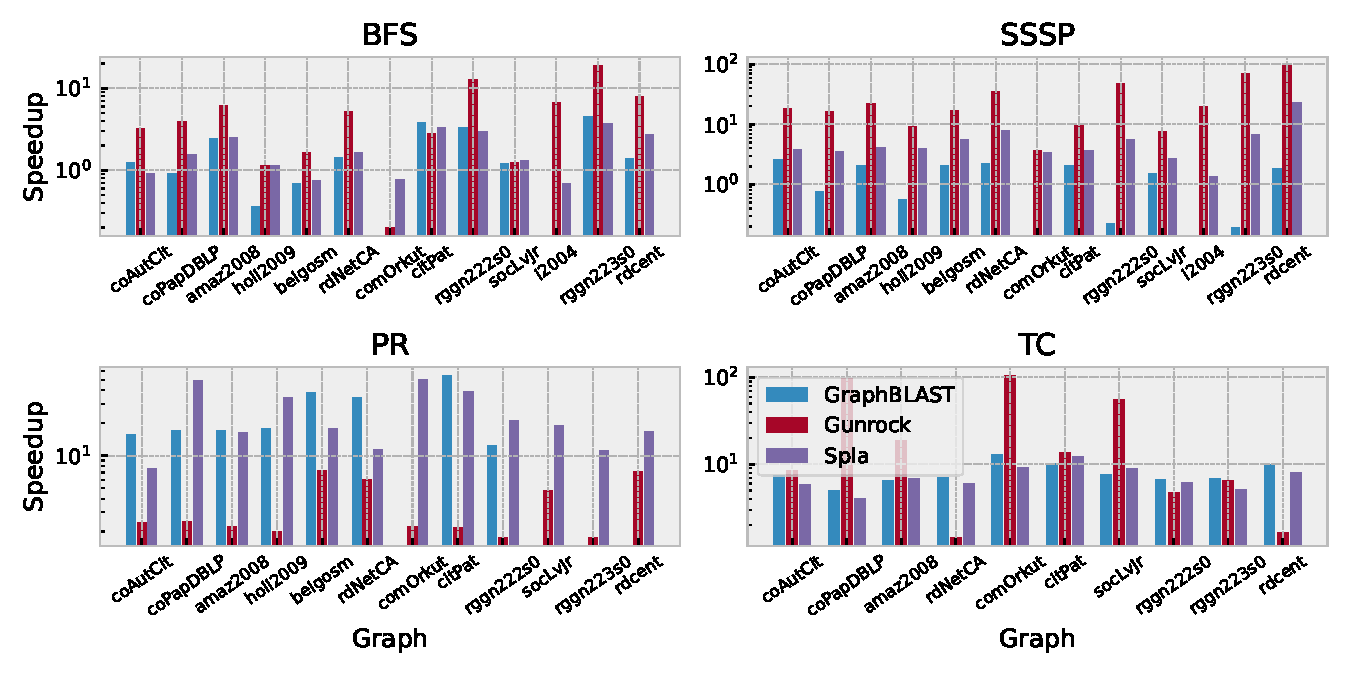
\includegraphics[width=1.0\textwidth]{figures/rq1_rel.pdf}
\end{minipage}
\begin{minipage}[t]{1.0\textwidth}
    \textbf{Tools:} Gunrock~\cite{7967137}, GraphBLAST~\cite{yang2019graphblast}, Spla and LaGraph~\cite{szarnyas2021lagraph} as a baseline.\\
    \textbf{Configuration}: Ubuntu 20.04, 3.40Hz Intel Core i7-6700 4-core CPU, DDR4 64Gb RAM, Nvidia GeForce GTX 1070 dedicated GPU with 8Gb on-board VRAM.
\end{minipage}
\vspace{-0.1cm}
}

\setlength{\tabcolsep}{5pt}
\headerbox{Evaluation: Scalability on different GPUs}{name=rq2,span=7,column=5,row=3,below=rq1}{
\begin{minipage}[b]{1.0\textwidth}
    \vspace{0pt}
    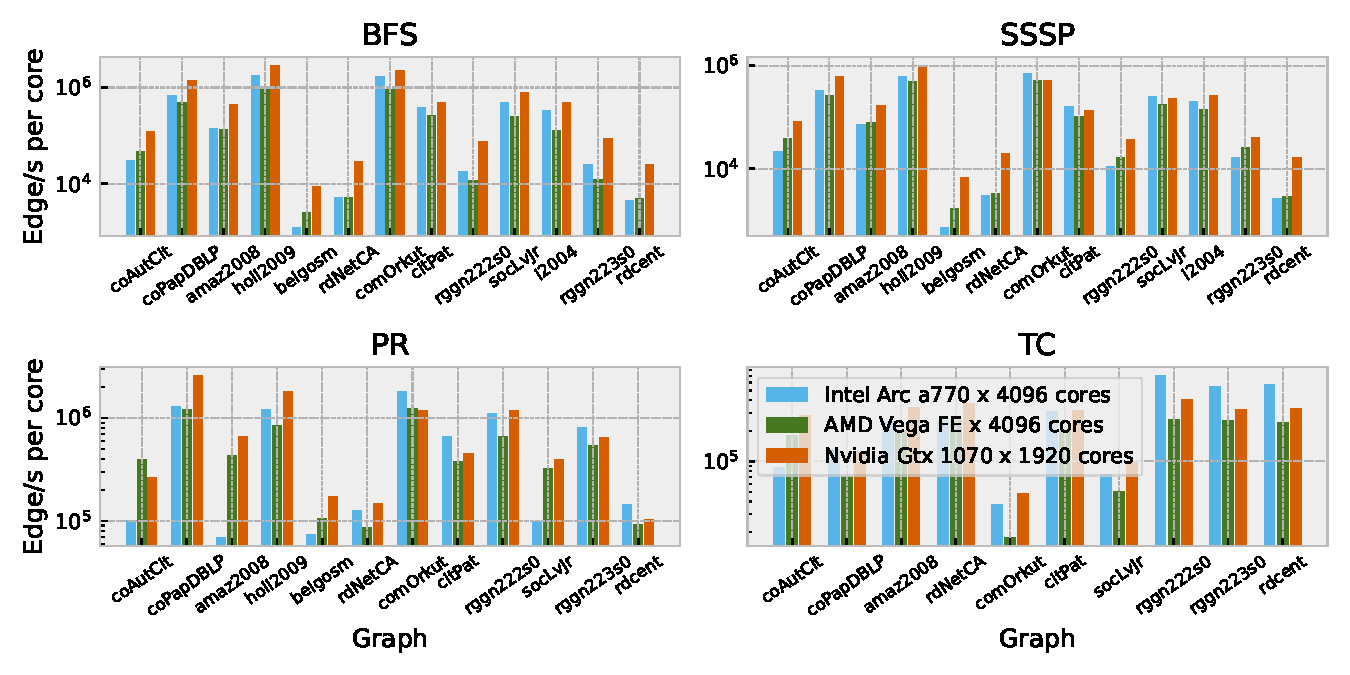
\includegraphics[width=1.0\textwidth]{figures/rq2_cores.pdf}
\end{minipage}
\begin{minipage}[t]{1.0\textwidth}
    \textbf{Configuration}: Ubuntu 20.04, 3.40Hz Intel Core i7-6700 4-core CPU, DDR4 64Gb RAM, Nvidia GeForce GTX 1070 dedicated GPU with 8Gb VRAM, Intel Arc A770 flux dedicated GPU with 8GB VRAM and or AMD Radeon Vega Frontier Edition dedicated GPU with 16GB VRAM.
\end{minipage}
\vspace{-0.1cm}
}

\headerbox {Motivating Example}
{name=example,column=0,span=5, row=2, below=problem}
{
\begin{minipage}[b]{1.0\textwidth}
    \vspace{0pt}
    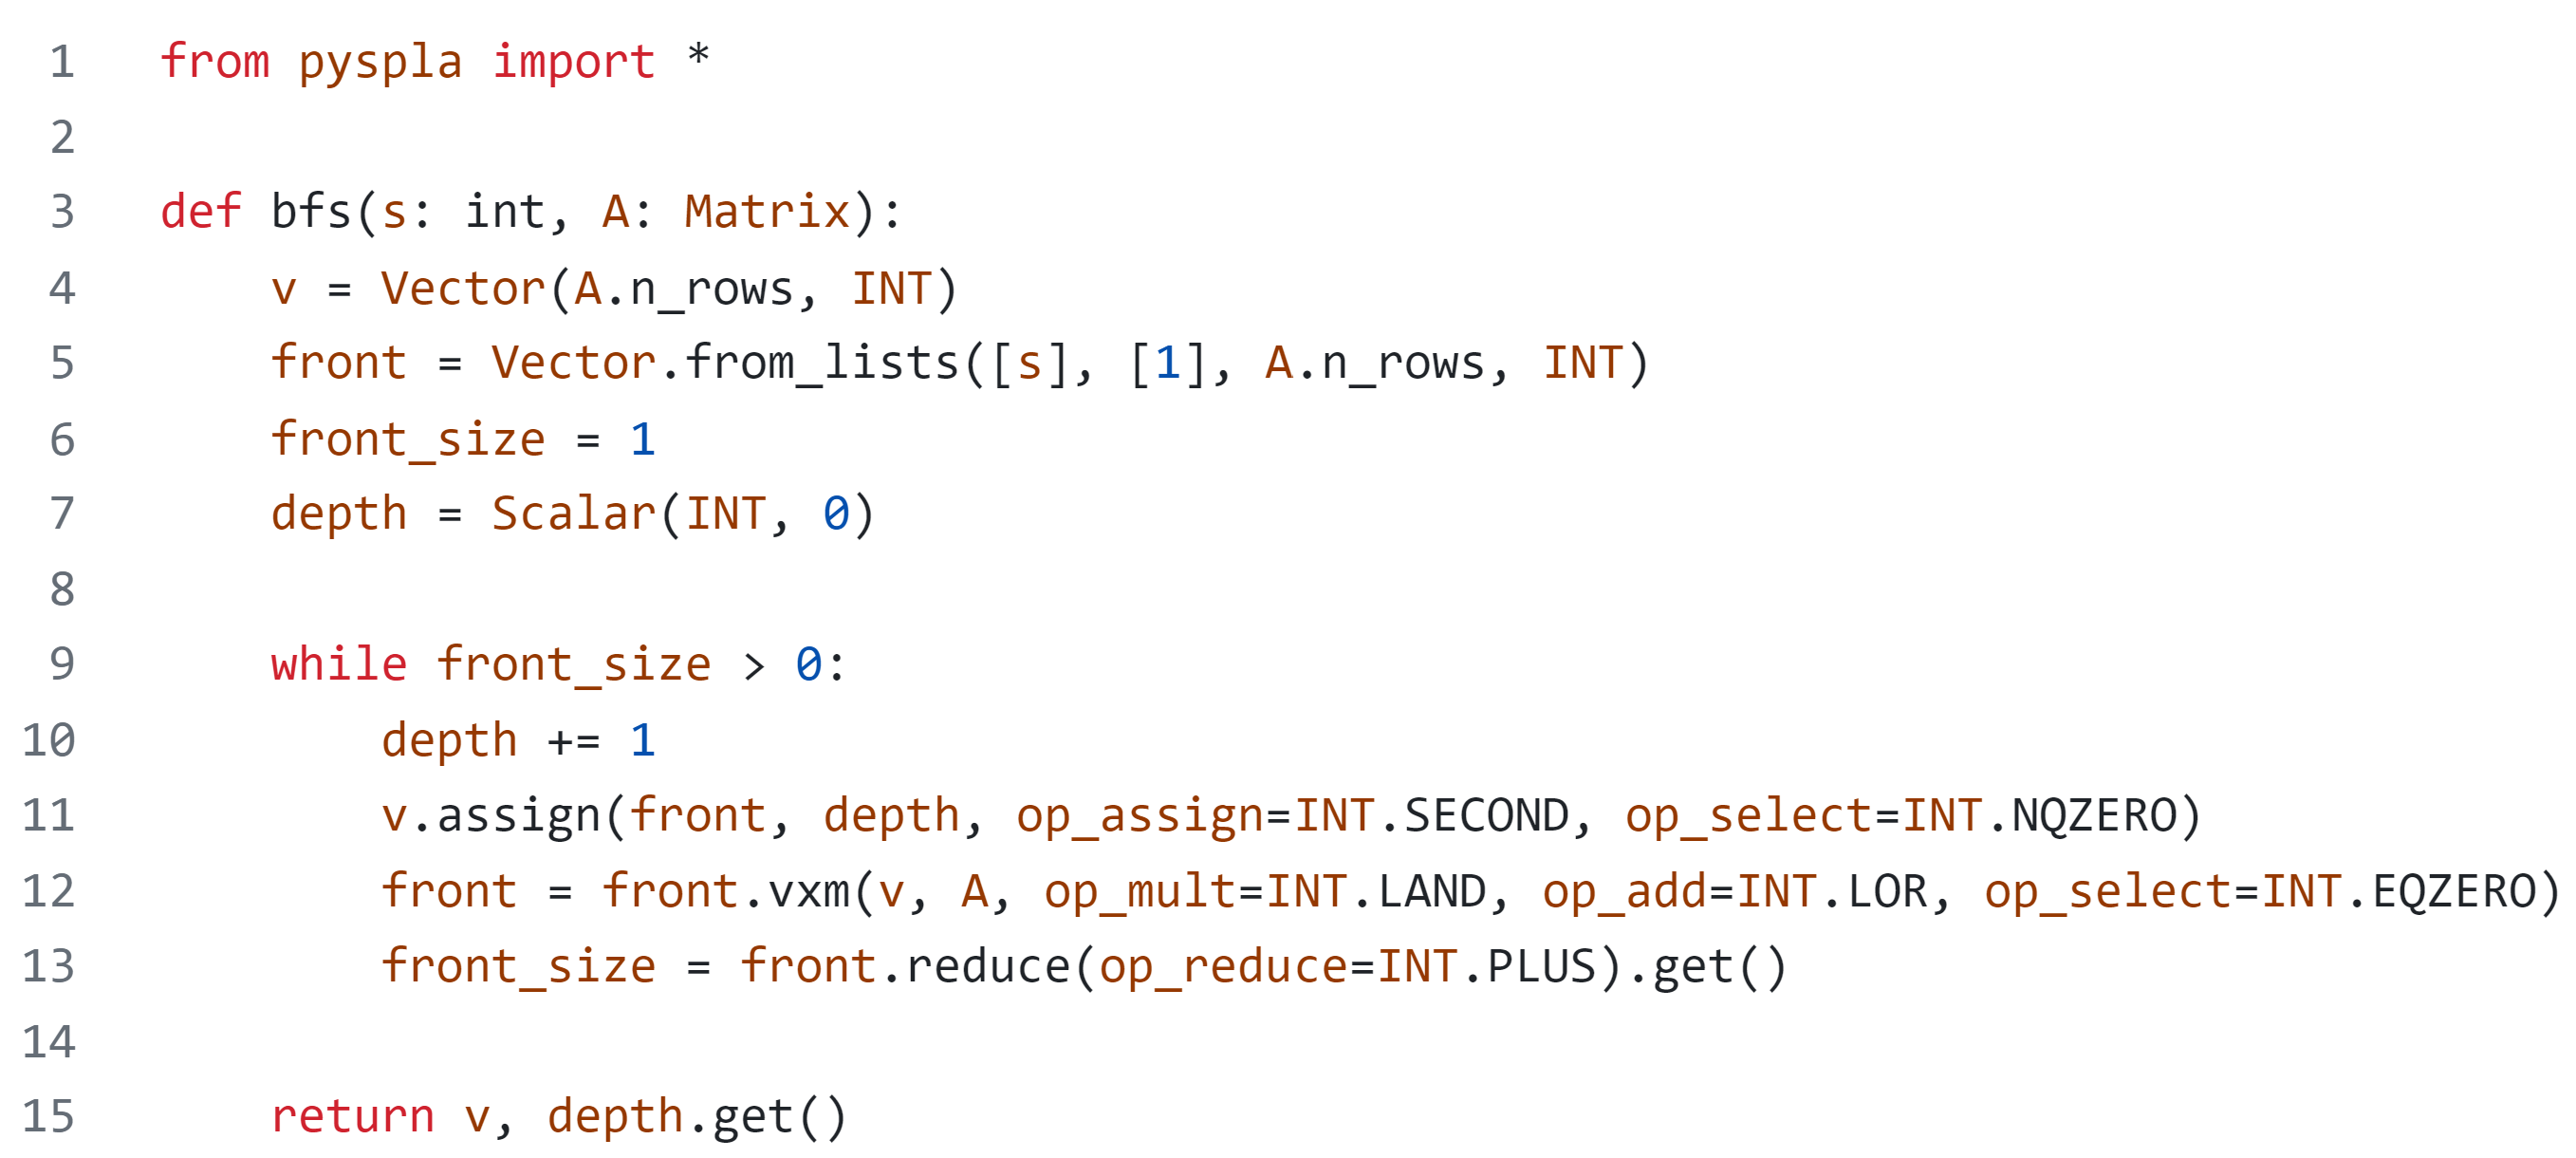
\includegraphics[width=\textwidth]{figures/spla_bfs.png}
\end{minipage}
\begin{minipage}[t]{1.0\textwidth}
    \textbf{Push-only BFS} implementation with out of the box \textbf{GPUs acceleration} using \textbf{pyspla} package API available at PyPI.
\end{minipage}
}

\headerbox {Implementation}
{name=implementation,column=0,span=5, row=3, below=example}
{
Spla implemented using the C++17 language and vendor-agnostic OpenCL 1.2 for GPU specific computations. General optimizations:

\begin{itemize}
    \item \textbf{K-way merge-based} \textit{vxm} operation~\cite{7284398:spvspm}.
    \item \textbf{Push-pull} and \textbf{early-out}~\cite{https://doi.org/10.48550/arxiv.1804.03327:pushpull}.
    \item \textbf{Masking} of reached vertices~\cite{yang2019graphblast}.
    \item \textbf{Sparse-dense} storage switch~\cite{yang2019graphblast}.
\end{itemize}
}

\headerbox {OpenCL Specifics}
{name=opencl,column=0,span=5, row=3, below=implementation, bottomaligned=rq2}
{
Auxiliary functionality and optimizations to reduce mostly OpenCL CPU-side driver overhead:
\begin{itemize}
    \item Run-time compiled \textbf{kernels cache} with a robin hood hash map for fast look-ups.
    \item In-place \textbf{unique kernel key} string constriction. 
    \item Kernel code compilation with \textbf{user-defined} functions using simple text preprocessing.
    \item \textbf{Custom linear allocator} based on sub-buffer mechanism for temporary small ($\leq1\textit{MiB}$) allocations.
    \item \textbf{Custom auxiliary} operations, such as \textit{sort}, \textit{reduce}, \textit{scan}.
\end{itemize}
}

\headerbox {\smaller{Contact Us}}{name=contact,column=0,span=5,below=opencl}{
\small
\begin{minipage}[t]{0.75\textwidth}
  \vspace{0pt}
Our team:
\begin{itemize}
  \item Semyon Grigorev: \href{mailto:s.v.grigoriev@spbu.ru}{s.v.grigoriev@spbu.ru}
  \item Egor Orachev: \href{mailto:egor.orachev@gmail.com}{egor.orachev@gmail.com}
\end{itemize}

\end{minipage}
~
\begin{minipage}[t]{2cm}
  \vspace{0pt}

\includegraphics[width=2cm]{figures/spla_qr.png}
\end{minipage}

}

\headerbox {\smaller{Acknowledgments}}{name=ack,column=0,span=5,below=contact}{
\small
We would like to thank Huawei Technologies Co., Ltd for supporting this research. We are also grateful to our team and reviewers.
}


\headerbox{\smaller{References}}{name=references,column=5,span=7,below=rq2,,bottomaligned=ack}{

    \scriptsize % Reduce the font size in this block
    \renewcommand{\section}[2]{\vskip 0.05em} % Get rid of the default "References" section title
    \nocite{*} % Insert publications even if they are not cited in the poster
    \bibliographystyle{unsrt}
    \bibliographystyle{IEEEtran}
    \bibliography{biblio} % Use biblio.bib as the bibliography file
}

\end{poster}
\end{document}